%! TEX root = ./main.tex

%\documentclass[a4paper,14pt]{extreport}
 
\usepackage{extsizes}
\usepackage{cmap} % для кодировки шрифтов в pdf
\usepackage[T2A]{fontenc}
\usepackage[utf8]{inputenc}
\usepackage[russian]{babel}
\usepackage{tempora}
%\usepackage{pscyr}
 
\usepackage{graphicx} % для вставки картинок
\usepackage{amssymb,amsfonts,amsmath,amsthm} % математические дополнения от АМС
\usepackage{indentfirst} % отделять первую строку раздела абзацным отступом тоже
\usepackage[usenames,dvipsnames]{color} % названия цветов
\usepackage{makecell}
\usepackage{multirow} % улучшенное форматирование таблиц
\usepackage{ulem} % подчеркивания
 
\linespread{1.3} % полуторный интервал
%\renewcommand{\rmdefault}{ftm} % Times New Roman
\frenchspacing

\usepackage{fancyhdr}
\pagestyle{fancy}
\fancyhf{}
\fancyhead[R]{\thepage}
\fancyheadoffset{0mm}
\fancyfootoffset{0mm}
\setlength{\headheight}{17pt}
\renewcommand{\headrulewidth}{0pt}
\renewcommand{\footrulewidth}{0pt}
\fancypagestyle{plain}{ 
    \fancyhf{}
    \rhead{\thepage}}
\setcounter{page}{5} % начать нумерацию страниц с №5

\usepackage[tableposition=top]{caption}
\usepackage{subcaption}
\DeclareCaptionLabelFormat{gostfigure}{Рисунок #2}
\DeclareCaptionLabelFormat{gosttable}{Таблица #2}
\DeclareCaptionLabelSeparator{gost}{~---~}
\captionsetup{labelsep=gost}
\captionsetup[figure]{labelformat=gostfigure}
\captionsetup[table]{labelformat=gosttable}
\renewcommand{\thesubfigure}{\asbuk{subfigure}}

\usepackage{titlesec}
 
\titleformat{\chapter}[display]
    {\filcenter}
    {\MakeUppercase{\chaptertitlename} \thechapter}
    {8pt}
    {\bfseries}{}
 
\titleformat{\section}
    {\normalsize\bfseries}
    {\thesection}
    {1em}{}
 
\titleformat{\subsection}
    {\normalsize\bfseries}
    {\thesubsection}
    {1em}{}
 
% Настройка вертикальных и горизонтальных отступов
\titlespacing*{\chapter}{0pt}{-30pt}{8pt}
\titlespacing*{\section}{\parindent}{*4}{*4}
\titlespacing*{\subsection}{\parindent}{*4}{*4}

\usepackage{geometry}
\geometry{left=3cm}
\geometry{right=1.5cm}
\geometry{top=2.4cm}
\geometry{bottom=2.4cm}

%\usepackage{enumitem}
%\makeatletter
%    \AddEnumerateCounter{\asbuk}{\@asbuk}{м)}
%\makeatother
%\setlist{nolistsep}
%\renewcommand{\labelitemi}{-}
%\renewcommand{\labelenumi}{\asbuk{enumi})}
%\renewcommand{\labelenumii}{\arabic{enumii})}


\usepackage{tocloft}
\renewcommand{\cfttoctitlefont}{\hspace{0.38\textwidth} \bfseries\MakeUppercase}
\renewcommand{\cftbeforetoctitleskip}{-1em}
\renewcommand{\cftaftertoctitle}{\mbox{}\hfill \\ \mbox{}\hfill{\footnotesize Стр.}\vspace{-2.5em}}
\renewcommand{\cftchapfont}{\normalsize\bfseries \MakeUppercase{\chaptername} }
\renewcommand{\cftsecfont}{\hspace{31pt}}
\renewcommand{\cftsubsecfont}{\hspace{11pt}}
\renewcommand{\cftbeforechapskip}{1em}
\renewcommand{\cftparskip}{-1mm}
\renewcommand{\cftdotsep}{1}
\setcounter{tocdepth}{2} % задать глубину оглавления — до subsection включительно

%------------------------------------------------------------------------------
\newcommand{\empline}{\mbox{}\newline}
\newcommand{\likechapterheading}[1]{ 
    \begin{center}
    \textbf{\MakeUppercase{#1}}
    \end{center}
    \empline}

\makeatletter
    \renewcommand{\@dotsep}{2}
    \newcommand{\l@likechapter}[2]{{\bfseries\@dottedtocline{0}{0pt}{0pt}{#1}{#2}}}
\makeatother
\newcommand{\likechapter}[1]{    
    \likechapterheading{#1}    
    \addcontentsline{toc}{likechapter}{\MakeUppercase{#1}}}


\graphicspath{{./images}}

%----------- For Table -------------
\usepackage{tabularx}
%-----------------------------------

%------------------------------------------------------------------------------
 
%\begin{document}
%
%  \tableofcontents
%
%  \newpage
%  \likechapter{ВСТУПЛЕНИЕ}
%
%  \chapter{ТЕХНОЛОГИЯ PROGRAM SYNTHESIS}
%  \section{Вступление}
%  \begin{itemize}
%    \item Hellow
%    \item world
%  \end{itemize}
%  \begin{enumerate}
%    \item I
%    \item am
%    \item Kerl
%      \begin{enumerate}
%        \item I love buby
%      \end{enumerate}
%  \end{enumerate}
%\end{document}

%! TEX root = ../main.tex
\documentclass[a4paper,14pt,russian]{extreport}

\usepackage{extsizes}
\usepackage{cmap}             % для кодировки шрифтов в pdf
\usepackage[T2A]{fontenc}
\usepackage[utf8]{inputenc}
\usepackage[russian]{babel}
\usepackage{tempora}

\usepackage{graphicx}         % для вставки рисунков
\graphicspath{{./images}}
\usepackage{amssymb,amsfonts,amsmath,amsthm} % математические дополнения от АМС
\usepackage{indentfirst}      % отделять первую строку раздела абзацным отступом
\usepackage[usenames,dvipsnames]{color} % названия цветов
\usepackage{makecell}
\usepackage{multirow}
\usepackage{ulem}             % подчеркивание

\linespread{1.3}              % полуторный интервал
\frenchspacing

\usepackage{tabularx}
\usepackage{xltabular}

\usepackage{ragged2e}

%--------------- Page number ---------------  
\usepackage{fancyhdr}
\pagestyle{fancy}
\fancyhf{}
\fancyfoot[C]{\small \thepage}
\fancyheadoffset{0mm}
\fancyfootoffset{0mm}
%\setlength{\headheight}{17pt}
\renewcommand{\headrulewidth}{0pt}
\renewcommand{\footrulewidth}{0pt}
\fancypagestyle{plain}{ 
    \fancyhf{}
    \cfoot{\small \thepage}}
\setcounter{page}{5} % начать нумерацию страниц с №5
%-------------------------------------------  

%-------------- Captions -------------------  
\usepackage[tableposition=top]{caption}
\usepackage{subcaption}
\DeclareCaptionLabelFormat{gostfigure}{Рис. #2}
\DeclareCaptionLabelFormat{gosttable}{Таблица \Alph{appendixCounter}.#2}
\DeclareCaptionLabelFormat{gostsubfigure}{#2.}
\DeclareCaptionFormat{my_new_table_format}{#1#2#3}
%\DeclareCaptionFormat{my_table_format}{\hfill #1 \par #3}
\DeclareCaptionLabelSeparator{tabsep}{~---~}
\DeclareCaptionLabelSeparator{gost}{~}
\captionsetup{labelsep=gost}

\captionsetup[figure]{labelformat=gostfigure, singlelinecheck=off, 
                      justification=centering}

\captionsetup[subfigure]{labelformat=gostsubfigure}

\captionsetup[table]{singlelinecheck=off,
                     format=my_new_table_format,
                     justification=RaggedRight,
                     labelformat=gosttable,
                     labelsep=tabsep}

\renewcommand{\thesubfigure}{\asbuk{subfigure}}
%-------------------------------------------  

%------------- Title (headers) -------------  
\usepackage{titlesec}

\titleformat{\chapter}  % command 
    [block]             % shape
    {\filcenter}        % format
    {\textbf{\thechapter.}} % label
    {\wordsep}          % sep
    {\bfseries}         % before
    {}                  % after
 
\titleformat{\section}
    {\normalsize\bfseries\filcenter}
    {\thesection.}
    {\wordsep}
    {}

\titleformat{\subsection}
    {\normalsize\filcenter}
    {\thesubsection.}
    {\wordsep}
    {}

\titlespacing*{\chapter}{0pt}{-30pt}{15pt}
\titlespacing*{\section}{0pt}{10pt}{10pt}
\titlespacing*{\subsection}{0pt}{10pt}{10pt}
%-------------------------------------------  

%------------ Page indentation -------------
\setlength{\parindent}{1.27cm}
\usepackage{geometry}
\geometry{left=30mm}
\geometry{right=15mm}
\geometry{top=20mm}
\geometry{bottom=20mm}
%-------------------------------------------  


%------------ items lists -----------------
\usepackage{enumitem}
\makeatother
%\setlist{nolistsep, leftmargin=0pt, 
%        itemindent=\dimexpr\labelwidth+\labelsep\relax}
\setlist{nolistsep, leftmargin=0pt, labelindent=\parindent,
         listparindent=\parindent, labelwidth=10pt, itemindent=!}
%\renewcommand{\labelitemi}{---}


\makeatletter
\renewcommand*{\@alph}[1]{%
  \ifcase#1\or а\or б\or в\or г\or
    д\or е\or ж\or и\or к\or л\or м\or
    \v z\else\@ctrerr\fi
}
%\renewcommand*{\@Alph}[1]{%
%  \ifcase#1\or A\or B\or C\or\v C\or
%    D\or E\or F\or G\or H\or I\or J\or
%    K\or L\or M\or N\or O\or P\or R\or S\or\v S\or
%    T\or U\or V\or W\or X\or
%    Y\or Z\or\v Z\else\@ctrerr\fi
%}
\makeatother

\renewcommand{\theenumi}{\alph{enumi}}
\renewcommand{\theenumii}{\arabic{enumii}}


%-------------------------------------------  

%---------- table of contents --------------
\usepackage{tocloft}

\renewcommand{\cfttoctitlefont}{\normalsize\hspace{0.38\textwidth}
                                \bfseries}
\renewcommand{\cftbeforetoctitleskip}{-1em}
\renewcommand{\cftaftertoctitleskip}{1em}
\renewcommand{\cftchappagefont}{\normalsize\normalfont} % номер страницы у глав
\renewcommand{\cftchapfont}{\normalsize}
\renewcommand{\cftchapleader}{\cftdotfill{\cftsecdotsep}} % точки между главой и
                                                          % страницей
\renewcommand{\cftsecindent}{1em}
\renewcommand{\cftsubsecindent}{2em}
%\renewcommand{\cftsecaftersnum}{.}
%\renewcommand{\cftsubsecaftersnum}{.}
%\renewcommand{\cftsubsecfont}{\hspace{11pt}}
\renewcommand{\cftbeforechapskip}{0pt} % убирает разрыв между главами
\renewcommand{\cftparskip}{-1mm}
\renewcommand{\cftdotsep}{1}
\setcounter{tocdepth}{2} % задать глубину оглавления — до subsection включительно

\AtBeginDocument{\renewcommand{\contentsname}{Содержание}}

%-------------------------------------------  

\newcommand{\StdChapter}[1]{
      \stepcounter{chapter}
      \chapter*{\thechapter. #1}
      \addcontentsline{toc}{chapter}{\thechapter. #1}
}

\newcounter{appendixCounter}
\setcounter{appendixCounter}{0}
\newcommand{\StdAppendix}[2]{
  \clearpage
  \stepcounter{appendixCounter}
  \begin{center}
    \textbf{ Приложение \Alph{appendixCounter} }\\
    (#1)\\
    #2
  \end{center}
  \addcontentsline{toc}{chapter}{Приложение \Alph{appendixCounter} #2}
}

%------------ listings --------------------
\usepackage{listings}
\usepackage{xcolor}

\definecolor{codegreen}{rgb}{0,0.6,0}
\definecolor{codegray}{rgb}{0.5,0.5,0.5}
\definecolor{codepurple}{rgb}{0.58,0,0.82}
\definecolor{backcolour}{rgb}{0.95,0.95,0.92}

\lstdefinestyle{mystyle}{
    backgroundcolor=\color{backcolour},   
    commentstyle=\color{codegreen},
    keywordstyle=\color{magenta},
    numberstyle=\tiny\color{codegray},
    stringstyle=\color{codepurple},
    basicstyle=\ttfamily\footnotesize,
    breakatwhitespace=false,         
    breaklines=true,                 
    captionpos=b,                    
    keepspaces=true,                 
    numbers=left,                    
    numbersep=5pt,                  
    showspaces=false,                
    showstringspaces=false,
    showtabs=false,                  
    tabsize=2
}

\lstset{style=mystyle}
%------------------------------------------


%------- Appendix settings ----------
\usepackage{fancyhdr}
\usepackage{blindtext}


\fancypagestyle{apppages}{%
  \fancyhf{}
  \renewcommand{\headrulewidth}{0pt}
  \fancyhead[LE,RO]{Продолжение приложения \Alph{appendixCounter}}
}
%-----------------------------------



\begin{document}

  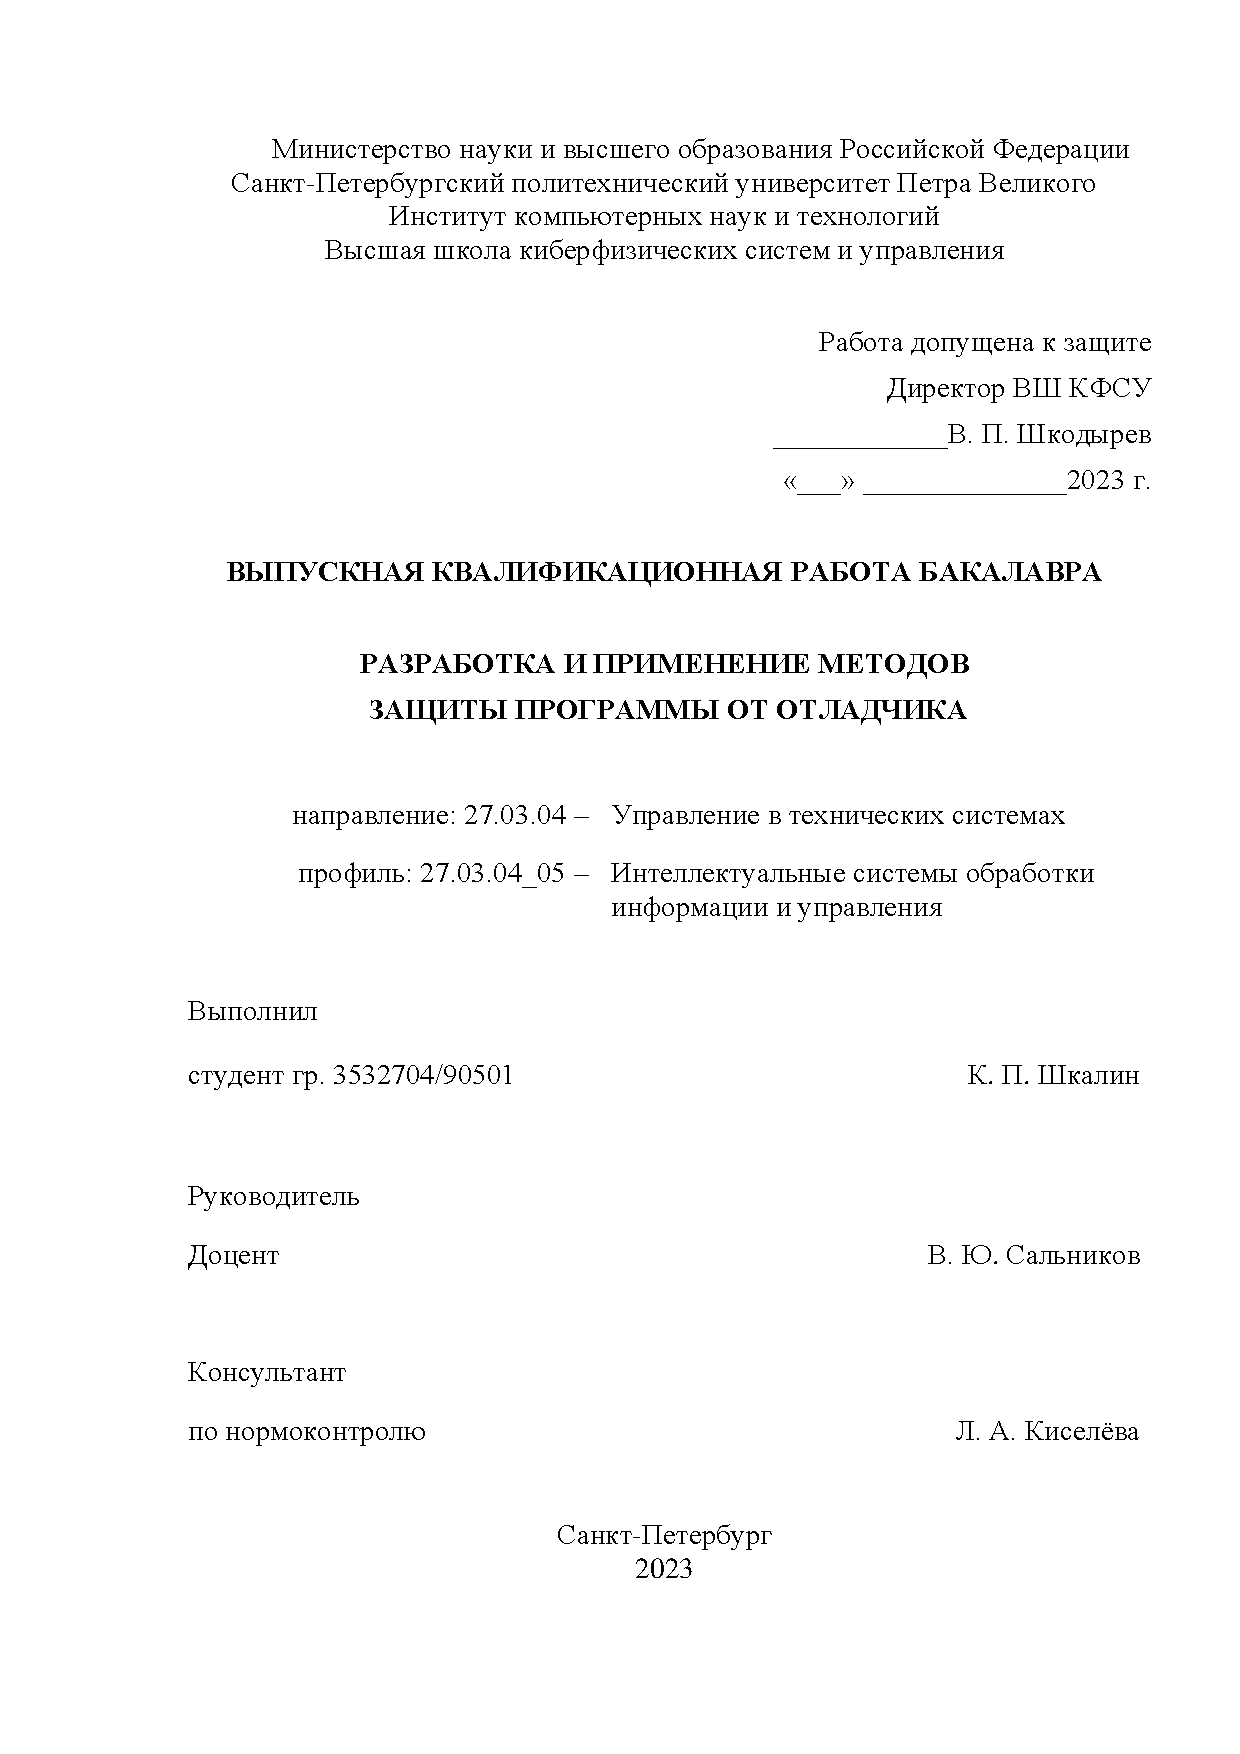
\includepdf[pages={1}]{title_page/title_page.pdf}
  
  %! TEX root = ../main.tex
\chapter*{Реферат}

\begin{center}
  \ztotpages\ с.\,, \totalfigures\ рис.\,, \totaltables\ таб.\,, 
  \totalappendixCounters\ прил.\\
  \vspace{4mm}
  \MakeUppercase{отладчик, защита программ, WinAPI, антиотладочные техники,
  ассемблер, дизассемблер, базовый адрес загрузки, контрольная сумма,
  PE-формат.}
\end{center}

В данной работе проектируется механизм защиты программы от изменения ее
исходного кода. Механизм основан на нахождении контрольной суммы секции кода.
Алгоритм нахождения контрольной суммы реализован на языке ассемблера. Для
проведения тестирования написана программа на языке C. Реализованы модули на
языке C++, предоставляющие набор функций для работы с секциями PE-файла.

%\vspace{3cm}
%{\let\clearpage\relax \chapter*{bar}}

\chapter*{Abstract}
\begin{center}
  \ztotpages\ p.\,, \totalfigures\ pic.\,, \totaltables\ tab.\,, 
  \totalappendixCounters\ app.\\
  \vspace{4mm}
  \MakeUppercase{debugger, program protection, WinAPI, anti-debugging techniques,
  assembler, disassembler, base load address, cyclic redundancy check,
  PE-format.}
\end{center}

In this paper, a mechanism is designed to protect the program from changing the
source code. The mechanism is based on finding the CRC of text section. The
algorithm for finding the CRC is implemented in assembly language. A program for
testing is developed in C. Modules are implemented in C++ language, providing a
set of functions for working with sections of a PE-file.

  \newpage

  \tableofcontents
  \thispagestyle{empty}
  \newpage

  \chapter*{Введение}
  %! TEX root=../main.tex

В современном мире многие  общественные процессы приобретают цифровую форму.
Так, например, банковские операции, беспилотные автомобили, умные дома,
хранилища информации о частной жизни людей имеют программно-информационные
аспекты. В связи с этим становится очевидной актуальность обеспечения
информационной безопасности. 

Зачастую злоумышленники получают доступ к конфиденциальным данным по средствам
нахождения уязвимостей в программном обеспечении. Также злоумышленники могут
изменять исходный код программного обеспечения для устранения частей, отвечающих
за защиту, с целью дальнейшего незаконного распространения данной программы. И в
первом, и во втором случае применяется программа, называемая отладчиком.
Изначально разработанные для упрощения процесса поиска ошибок в собственных
программах, отладчики получили широкое распространение как инструмент взлома. 

На российском рынке представлены две крупные организации, работа которых
посвящена проблеме информационной безопасности:
\begin{itemize}
  \item Лаборатория Касперского --- международная компания, работающая в сфере
    информационной безопасности и цифровой приватности.
  \item Hex-Rays, основанная Ильфаком Гульфановым, занимается разработкой
    инструментов двоичного анализа для рынка IT-безопасности.
\end{itemize}

Эти компании выпускают комплексные системы защиты, не интегрирующиеся в
программу, а выступающие сторонними модулями. Для обеспечения
защиты от угроз со стороны отладчика было принято решение
разработать метод, который сможет как обеспечить обнаружение факта работы
программы под отладчиком, так и препятствовать самому процессу отладки.

%В свою очередь целью данной работы является разработка методов обеспечения
%защиты программы от взлома отладчиком. Данные методы должны как обеспечивать
%обнаружение факта работы программы под отладчиком, так и препятствовать самому
%процессу отладки.

\textit{Целью данной бакалаврской работы} является разработка системы
безопасности программного обеспечения от повреждения отладчиком.  В связи с этим
были поставлены следующие задачи:

\begin{enumerate}
  %\item Изучить внутреннее устройство программы отладчика.
  \item изучить алгоритм действия отладчика;
  \item разработать алгоритм защиты от отладчика;
  \item реализовать полученный алгоритм, обеспечив при этом достаточный
    уровень скрытности;
  \item провести тестирование полученной системы защиты.
\end{enumerate}

  \addcontentsline{toc}{chapter}{Введение}

  \StdChapter{Общие сведения о работе отладчика}
  Данная глава включает в себя общие сведения о работе отладчика, которые затем 
  будут  использованы для защиты программ от него же. Помимо этого 
  рассматривается структура исполняемого файла в операционной системе Windows.
  \section{Принципы работы отладчика}
Отладчик~--- это программа, которая упрощает разработку программного
обеспечения, предоставляя разработчику способы поиска ошибок. Обычно функционал
отладчика предоставляет следующие возможности:
\begin{itemize}
  \item поставить точку останова. Например, пометить инструкцию, дойдя до
    которой, программа должна остановить свое выполнение и передать управление
    отладчику;
  \item трассировать программу. То есть, последовательно выполнять инструкции, и
    после каждой останавливать выполнение программы, и передавать управление
    отладчику;
  \item отобразить состояние регистров процессора на момент останова;
  \item отобразить состояние стека процесса на момент останова.
\end{itemize}

Возможности, предоставляемые отладчиком, могут быть использованы
злоумышленниками для изучения уязвимостей программного обеспечения, а также
обхода ограничений и защиты.  Для лучшего понимания способов защиты от отладчика
рассмотрим, как работает каждая предоставляемая им возможность более
подробно.

Отладчик может самостоятельно запустить отлаживаемый процесс. В рассматриваемой
системе Microsoft Windows для этого нужно вызвать функцию \verb!CreateProcess!
с указанием ей в качестве параметра \verb!fdwCreate! константы
\verb!DEBUG_PROCESS!. Также отладчик может подключиться к уже работающему
процессу. Для этого ему необходимо получить идентификатор процесса при помощи
функции \verb!OpenProcess!, после чего вызвать \verb!DebugActiveProcess! и, таким
образом, подключиться к нему.  Как правило, отладчик открывает процесс с доступом
на чтение и запись в виртуальную память процесса.

Затем отладчик в цикле обрабатывает события отладки, используя функцию
\verb!WaitForDebugEvent!. После завершения обработки очередного события отладки
вызывает функцию \verb!ContinueDebugEvent!. Общую схему работы отладчика можно
представить следующим образом:
\begin{verbatim}
  CreateProcess("FileName.exe", ..., DEBUG_PROCESS, ...); 
  for (;;) {
    WaitForDebugEvent(&dbgEv, INFINITE);
    switch(dbgEv.dwDebugEventCode) 
    {
    case EXCEPTION_DEBUG_EVENT:
    ...
    }
    ContinueDebugEvent( dbgEv.dwProcessId,
                        dbgEv.dwThreadId,
                        dwContinueStatus );
  }
\end{verbatim}

Перейдем к рассмотрению конкретных возможностей предоставляемых отладчиком.

  %! TEX root = ../main.tex

\section{Трассировка}
Трассировка~--- последовательное выполнение программы, при котором после каждой
инструкции управление передается отладчику. В этом режиме программист может
детально отследить изменения значений всех параметров процесса. Обеспечение
режима пошагового выполнения программы предусмотрено на аппаратном уровне.

В архитектуре x86 есть регистр флагов (EFLAGS), состоящий из 32-х бит, каждый из
которых отображает состояние процессора (рис.  \ref{fig:eflags}).
\begin{figure}[htpb]
  \centering
  \includegraphics[width=0.8\textwidth]{eflags.jpg}
  \caption{Регистр флагов процессора}
  \label{fig:eflags}
\end{figure}
Восьмой из них является флагом трассировки (trap flag). Если этот флаг равен 1,
то процессор будет выполнять прерывание с номером 1 после каждой инструкции. При
выполнении прерывания 1 процессор выполняет передачу управления в обработчик
прерывания, который помещает состояние всех регистров процессора в стек, после
чего передает необходимую информацию отладчику. Обработчик прерывания в конце
своей работы может либо оставить флаг трассировки равным 1, либо перевести его
значение в 0.

Пример установки флага трассировки:
\begin{verbatim}
  pushf                    ; Помещаем регистр флагов в стек
  mov EBP, ESP             ; Сохраняем адрес вершины стека
  or  WORD PTR[EBP], 0100h ; Устанавливаем флаг TF
  popf                     ; Восстанавливаем регистр флагов
\end{verbatim}
Соответственно, чтобы снять флаг трассировки достаточно заменить инструкцию
\verb!or! на инструкцию:
\begin{verbatim}
  and  WORD PTR[EBP], FEFFh
\end{verbatim}

Таким образом, можно заметить, что при проведении трассировки исходный код
отлаживаемой программы никак не меняется.

  %! TEX root = ../main.tex

\section{Точки останова}
Точка останова~--- место в коде программы, дойдя до которого процессор должен
прервать выполнение программы и передать управление отладчику. После этого
программист может просмотреть параметры состояния программы, поставить или
убрать другие точки останова или запустить трассировку. Точки останова бывают
двух типов: программные и аппаратные.

Рассмотрим принцип работы каждой из них.

\subsection{Программные точки останова}
Программные точки останова реализованы следующим образом. Когда программист
ставит точку останова на какой-либо инструкции, отладчик запоминает данную
инструкцию у себя в памяти, а затем заменяет данную инструкцию на 
\begin{verbatim}
  int 3 ; Генерация программного прерывания
\end{verbatim}
Таким образом, когда процессор доходит до данной инструкции, возбуждается
прерывание, управление переходит в обработчик прерывания, откуда затем
информация передается в отладчик. 

Инструкция \verb!int 3! имеет специальный однобайтовый код операции
(\verb!0xCC!), в то время, как обычно прерывания имеют двухбайтовый код
операции: \verb!int x!~$\to$~\verb!0xCD x!. Это связано с тем, что может
потребоваться заменить в коде однобайтовую операцию, например команду инкремента
\verb!inc!. В таком случае, если бы инструкция замены была больше одного
байта, то повреждалась бы следующая инструкция. Это в свою очередь накладывает
дополнительные расходы в ситуации, когда требуется из точки останова произвести
трассировку.

Как видно, установка программной точки останова изменяет исходный код
программы.

\subsection{Аппаратные точки останова}
В архитектуре x86 есть шесть регистров предназначенных специально для отладки.
Именуются они \verb!DR0...DR7!, при этом регистры \verb!DR4! и \verb!DR5! не
используются. Данные регистры позволяют устанавливать точки останова с
различными условиями. Также они ялвяются привилегированным ресурсом,
следовательно инструкции, устанавливающие данные регистры, могут выполняться
только с нолувого уровня защиты.

Регистры с \verb!DR0! по \verb!D3! содержат линейные адреса точек останова,
каждая из которых связана с условием остановки. Условия определены в регистре
\verb!DR7!.

В регистре \verb!DR6! содержится статус отладки. Он позволяет отладчику
оределить, какие условия отладки возникли. Первые четыре бита указывают, какая
из четырех точек останова в регистрах \verb!DR0...DR3! сработала. Бит 13
указывает, что следующая инструкция обращается к регистрам отладки. Бит 14
указывает на пошаговое выполнение (включает Trap Flag в регистре EFLAGS). 

Регистр \verb!DR7! предназначен для управления процессом отладки, он позволяет
выборочно включать условия остановки для точек останова в регистрах
\verb!DR0...DR3!. Есть два режима включения регистра: локальный (биты 0, 2, 4,
6) и глобальный (биты 1, 3, 5, 7). При локальном включении процессор сбрасывает
условия остановки при каждом переключении задачи. При глобальном включении
условия остановки не сбрасываются, а следовательно они используются для всех
задач. Биты 17:16; 21:20; 25:24 и 29:28 позволяют установить следующие условия
срабатывания точек останова:
\begin{itemize}
  \item \verb!00b! --- При выполнении инструкции.
  \item \verb!01b! --- При записи данных.
  \item \verb!10b! --- При обращении к порту ввода/вывода.
  \item \verb!11b! --- Чтение и запись данных.
\end{itemize}

Как можно заметить, установка аппаратных точек останова никак не меняет исходный
код программы.

  %! TEX root = ../main.tex

\section{Наиболее распространенные отладчики}
Для лучшего противодействия отладчику полезно рассмотреть какие отладчики
используются на сегодняшний день. Исходя из этой информации можно организовать
простой способ защиты. Например, программа в процессе работы может просмотреть
процессы запущенные в системе, и, если среди них встретится какой-либо знакомый
отладчик, программа может изменить свое поведение или просто прервать
выполнение.

\subsection{SoftICE}
Наиболее важным свойством отладчика SoftICE является то, что он работает на
нулевом кольце защиты.

В архитектуе x86 есть три кольца защиты (ring-1, 2, 3).
Данные кольца предназначены для ограничения взаимодействия выполняющихся
программ между собой и с операционной системой. Как правило, на нулевом кольце
защиты выполняется сама операционная система, которая одна имеет доступ ко всем
привилегированным операциям. Рассматриваемый отладчик также располагается на
нулевом кольце защиты, что позволяет ему отлаживать не только пользовательские
приложения, но также драйвера и саму операционную систему.

Поддержка отладчика разработчиками прекратилась 11 июля 2007 года.

\subsection{IDA Pro}
IDA Pro --- интерактивный дизассемблер и универсальный отладчик. 

Дизассемблер --- программный инструмент, позволяющий получить из машинного кода
код на языке ассемблера. По принципу работы они делятся на пассивные и
интерактивные. Автоматические предоставляют пользователю готовый листинг
программы, а интерактивные позволяют на ходу изменять правила по которым
производится трансляция.

Как дизассемблер IDA Pro способен создавать карты выполнения фрагментов
программы, делая полученный код ассемблера еще более понятным человеком.В
качестве отладчика IDA Pro охватывает все рассмотренные ранее возможности
отладки, обеспечивает доступ ко всем сегментам пространства памяти процесса, а
также обеспечивает подробную визуализацию.

Проект активно поддерживается и развивается.

\subsection{WinDBG}
WinDBG --- отладчик предоставляемый фирмой Microsoft, предназначенный специально
для работы в операционной среде Windows. Является более мощной альтернативой
широко применяемому отадчику Visual Studio Debugger. Может использоваться как
отладчик режима. Имеет поддержку сторонних расширений. На данный момент является
одним из самых применяемых, благодаря своей универсальности.

\subsection{OllyDbg}
OllyDbg --- отладчик уровня приложений (ring-3). Помимо поддержки всех
рассматриваемых ранее возможностей отладки, больш\'ая часть мощности OllyDbg
заключается в расширениях, которые разрабатывают пользователи этого отладчика и
выкладывают в сеть Internet. OllyDbg имеет бесплатное распространение, а также
не требует установки. 

Для тестирования разработанных методов в данной работе применяется именно этот
отладчик.

  %! TEX root = ../main.tex

\section{PE формат}
Исполняемые файлы в системе Windows имеет общую сигнатуру, называемую
PE (Portable Executable). В PE формате содержится различная информация о
исполняемом файле, как например: таблицы импорта и экспорта, информация о
различных секциях, точка входа и так далее. Структура PE формата представлена на
рисунке \ref{fig:PE}.
\begin{figure}[htb]
  \centering
  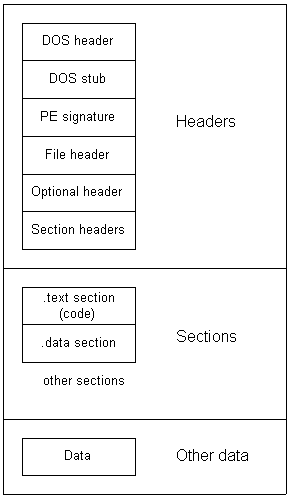
\includegraphics[width=0.45\textwidth]{PE.png}
  \caption{Формат PE}
  \label{fig:PE}
\end{figure}

Рассмотрим те части PE формата, которые будут использованы в данной работе.
Первым идет MS-DOS заголовок, первыми двумя байтами которой является сигнатура
"MZ". Большая часть полей данного заголовка предназаначены для запуска из-под
DOS. Для дальнейшей работы, кроме проверки сигнатуры, потребуется поле
\verb!e_lfanew!, в котором содержится указатель на начало PE-заголовока.

PE-заголовок также имеет свою сигнатуру, которую необходимо проверить на
корректность, а именно четыре байта "PE\textbackslash0\textbackslash0". В данном
разделе хранится количество секций \verb!NumberOfSection!, а также размер
идущего за следующим опционального заголовка в байтах
\verb!SizeOfOptionalHeader!.

Далле расположен опциональный заголовок. Данный раздел содежит смещение адреса
входа относительно базового адреса загрузки файла --- \texttt{AddresOfEntryPoint},
рекомендуемый базовый адрес загрузки файла \verb!ImageBase!, количество
элементов в таблице \verb!DATA_DIRECTORY! --- \verb!NumberOfRvaAndSizes!.
\verb!DATA_DIRECTORY! представляет собой таблицу, каждый элемент которой
представляет из себя структуру из двух полей, а именно виртулього адреса тех
данных, на который указывает данный элемент, и их размер. 

Далее идет таблица секций. Для каждой секции в этой таблице приведена следующая
информация:
\begin{itemize}
  \item \verb!Name! --- имя секции. 
  \item \verb!VirtualAddress! --- виртуальный адрес секции в памяти.
  \item \verb!PointerToRawData! --- указатель на данные в файле.
  \item \verb!VirtualSize! --- размер, занимаемый секцией в памяти.
  \item \verb!Characteristics! --- свойства секции. Так, например, секция,
    которую можно запустить на выполнение должна обладать свойством
    \verb!IMAGE_SCN_CNT_CODE!.
\end{itemize}


  \StdChapter{Проектирование методов защиты от отладчика}
  Данная глава посвящена разбору методов, которые могут обнаружить отладчик или
  препятствовать процессу отладки. Также в этой главе разбираются задачи,
  которые необходимо решить при реализации метода с подсчетом контрольной суммы.
  %! TEX root = ../main.tex

\section{Обзор методов защиты от отладчика}
Как было отмечено в предыдущей главе, отладчик может предоставить
злоумышленникам большой инструментарий по взлому программы. Следовательно,
необходимо разработать механизм, который будет препятствовать работе отладчика.
Рассмотрим несколько способов обнаружить, что программа работает под отладчиком.

\subsection{Возможности предоставляемые операционной системой}
Операционная система Windows предоставляет следующие функции:
\begin{verbatim}
  BOOL IsDebuggerPresent();
  BOOL CheckRemoteDebuggerPresent(
      [in]    HANDLE hProcess,
      [out]   PBOOL pbDebuggerPresent );
\end{verbatim}

Первая функция позволяет понять находится ли процесс, который совершил вызов,
под отладчиком. Если процесс выполняется под отладчиком, то функция вернет
ненулевое значение, а иначе вернет ноль.

Вторая функция принимает первым параметром дескриптор процесса, а вторым
указатель на переменную типа \verb!BOOL!, в которую функция занесет \verb!TRUE!,
если указанный процесс выполняется под отладчиком, или \verb!FALSE!, если
отладчика нет. Функция возвращает ненулевое значение в случае успеха и ноль,
если произошла ошибка.

Недостаток метода основанного на данных функциях заключается в его очевидности.
Большинство отладчиков имеют расширения, которые позволяют обойти проверку
данных функций.

\subsection{Замер времени выполнения}
При отладке программы время выполнения инструкций многократно увеличивается, так
как программа выполняется пошагово. Можно замерить время выполнения участка
кода, и если время выполнения этого участка окажется сильно больше планируемого
при штатной работе (например несколько секунд), то можно сделать вывод, что
программа выполняется под отладчиком.

Есть несколько доступных способов замерить время выполнения участка программы:
\begin{itemize}
  \item Использовать инструкцию \verb!rdtsc!. Эта инструкция считывает текущее
    значение счетчика меток времени процессора (64-битный \verb!MSR!) в регистры
    \verb!EDX:EAX!. В регистр \verb!EDX! загружаются старшие 32 бита \verb!MSR!,
    а в регистр \verb!EAX! младшие 32 бита. В коде такую проверку можно
    представить следующим образом:
    \begin{verbatim}
    rdtsc
    xchg  esi, eax
    mov   edi, edx
    rdtsc
    sub   eax, esi
    subb  edx, edi
    jne   _being_debugged
    cmp   eax, elapsed ; elapsed содержит максимальное
                       ; время выполнения участка кода
    jnbe  _being_debugged
    \end{verbatim}

  \item Использовать API операционной системы Windows:
    \begin{itemize}
      \item Функции работы со временем \verb!GetSystemTime! или
        \verb!GetLocalTime!. В этом случае придется переводить полученной время
        в 8-байтовое число, чтобы можно было посчитать разницу между двумя
        значениями времени.
      \item Функции счетчики, которые возвращают количество миллисекунд
        (микросекунд) с момента запуска системы. Это соответственно функции
        \verb!GetTickCount! и \verb!QueryPerformanceCounter!. При использовании
        этих функций переводить время в число не требуется, что делает их более
        предпочтительными.
    \end{itemize}

  \item Прочитать время с платы CMOS. Но, чтобы получить доступ к портам
    ввода/вывода, необходимо установить соответствующий драйвер.
\end{itemize}

\subsection{Нахождение контрольной суммы участка кода}
Данная работа посвящена реализации самого трудоемкого и сложного метода защиты
от отладчика. Суть метода заключается в том, чтобы посчитать контрольную сумму
участка кода программы и занести в одну из переменных. При необходимости
проверки наличия отладчика программа будет проверять соответствует ли текущее
значение контрольной суммы кода сохраненному ранее значению. 

Преимуществом данного метода является то, что он не только позволяет обнаружить
отладчик, но и защищает программу от любых изменений вносимых в ее код. Также
в работе будет рассмотрен способ нахождения контрольной суммы без обращения к
системным вызовам, что дополнительно усложняет нахождение участка защиты.

Рассмотрим проблемы и особенности, с которыми предстоит столкнуться при
реализации данного метода.

  %! TEX root = ../main.tex

\section{Нахождение необходимой секции в памяти}
\label{sec:finding}

Разрабатываемый метод будет вычислять контрольную сумму секции кода программы.
Путем несложных изменений можно адаптировать метод так, чтобы он искал
контрольную сумму секции данных, ресурсов или любой другой секции. Для этого
необходимо найти начало и размер конкретной секции в памяти. Чтобы решить эту
задачи можно воспользоваться знаниями об устройстве PE формата. 

Для нахождения нужной секции программа будет выполнять следующий алгоритм:
\begin{enumerate}[label=\arabic*.]
  \item Прибавить к базовому адресу загрузки 60 и прочитать четыре байта по этому
    адресу. По смещению в шестьдесят байт от базового адреса загрузки находится
    относительный виртуальный адрес PE-заголовка.
    
  \item Перейти к PE-заголовку, прибавив к базовому адресу прочитанные четыре
    байта. 

  \item Считать количество секций, которое содержится по смещению в 6 байт от
    PE-заголовка в двухбайтовом слове.

  \item По смещению в 20 байт от PE-заголовка находится двухбайтовое число, в
    котором содержится размер опционального заголовка. Это значение нам нужно
    для того, чтобы перейти к разделу секций.

  \item После этого необходимо перейти к опциональному заголовку, который
    находится по смещению в 24 байта от PE-заголовка. 

  \item \label{item:dd_offset} По смещению в 96 байт от опционального
    заголовка находится массив 8-ми байтовых значений. Первые четыре байта
    содержат адрес секции, а вторые четыре байта содержат размер секции. Пятый
    элемент этого массива соответствует таблице базовых релокаций, которая нам
    понадобится при подсчете контрольной суммы. Эти значения необходимо
    сохранить.

  \item После этого необходимо перейти к разделу секций, прибавив к началу
    опционального заголовка его размер, полученный на 4 этапе.

  \item \label{item:dd_struct} Раздел секций представляет собой массив структур,
    в которых находится информация о всех секциях, которые есть в программе.
    Необходимо циклом пройти по всем элементам данного массива, пока не
    встретится структура интересующей нас секции. Определить необходимую
    структуру можно по по полю характеристик секции. Так, например, секция кода
    содержит характеристику \verb!IMAGE_SCN_CNT_CODE! (\verb!0x00000020!).

  \item При нахождении интересующей секции необходимо сохранить ее относительный
    виртуальный адрес и размер.

\end{enumerate}

В итоге проделанных действий мы будем иметь относительные виртуальные адреса и
размеры искомой секции и таблицы базовых релокаций.



  %! TEX root = ../main.tex

\section{Нахождение базового адреса загрузки}

Чтобы найти расположение нужной секции, нам также нужно знать базовый адрес
загрузки программы.

Самый очевидный способ получить базовый адрес загрузки --- это вызвать
соответствующую функцию Windows API. А именно, если вызвать функцию
\verb!GetModuleHandle! и в качестве параметра передать нулевой указатель, то
функция вернет переменную типа \verb!HMODULE!, значение которой будет
соответствовать базовому адресу загрузки программы.

Для нашей задачи такой подход имеет недостаток в виде системного вызова. Так как
отследить обращение к системным вызовам при помощи отладчика очень просто, такой
подход может поставить защиту под угрозу.

Чтобы получить базовый адрес загрузки программы без обращения к функциям API
Windows, обратимся к структуре PEB. PEB (process environment block) --- это
структура, которая содержит информацию о процессе, в памяти которого она
хранится. Процесс может получить доступ к этой структуре при помощи регистра fs
(для 64-битного процесса регистр gs). Получить адрес PEB можно, выполнив
следующий код:
\begin{verbatim}
  mov eax, fs:0x30
\end{verbatim}
После чего в регистре \verb!EAX! будет содержаться адрес PEB. По смещению в 8
байт в PEB хранится базовый адрес загрузки.

Таким образом можно получить базовый адрес загрузки без обращения к системным
вызовам.

  %! TEX root = ../main.tex

\section{Таблица базовых релокаций}

Как отмечалось ранее, операционная система Windows использует механизм ASLR.
ASLR (Address space layout randomization) --- это метод компьютерной
безопасности, предназначенный для предотвращения использования уязвимостей,
связанных с повреждением памяти. Данный прием может предотвратить простой
переход злоумышленника, например, к конкретной функции в памяти. ASLR случайным
образом упорядочивает позиции адресного пространства ключевых областей данных
процесса, включая базовый адрес загрузки, позиции стека, кучи и загружаемых
библиотек.

Из вышеизложенного следует, что адреса конкретных функций и переменных
невозможно определить до запуска программы. Следовательно, должен быть механизм
корректировки адресов в различных секциях программы. Например, необходимо
изменить все абсолютные адреса из инструкций \verb!jmp! в соответствии с
конкретным базовым адресом.

В системе Windows для этого в каждом исполняемом файле, который поддерживает
ASLR, есть таблица базовых релокаций. При помощи этой таблицы загрузчик
приложений Windows может скорректировать участки программы в соответствии с
адресом загрузки.

Таблица базовых релокаций содержит записи для всех исправлений в образе
программы. Общий размер таблицы содержится в опциональном заголовке. Вся таблица
разбита на блоки исправлений. Каждый блок содержит исправления для страницы
размера 4\,Кбайт и выровнен по 32-битной границе. 

Каждый блок исправлений начинается со структуры описанной в таблице
\ref{tab:fixup_block}.

\begin{table}[h!]
  \centering
  \caption{Структура блока исправлений}
  \label{tab:fixup_block}
  \begin{tabularx} {\textwidth} {
      | >{\raggedright \arraybackslash \hsize=.17\hsize}X 
      | >{\arraybackslash \hsize=.13\hsize}X
      | >{\arraybackslash \hsize=.25\hsize}X
      | >{\arraybackslash \hsize=.45\hsize}X|
    } 
    \hline 
    \textbf{Смещение} & \textbf{Размер} & \textbf{Поле} & \textbf{Значение} \\
    \hline 
    0 & 4 & Относительный виртуальный адрес страницы &
      Базовый адрес загрузки и относительный виртуальный адрес
      страницы прибавляется к каждому смещению в таблице, чтобы получить
      виртуальный адрес по которому необходимо провести исправление \\
    \hline
    4 & 4 & Размер блока исправлений &
      Общее количество байтов, занимаемых блоком исправлений, включая эту
      структуру.\\
    \hline
  \end{tabularx}  
\end{table}

После описанной структуры следуют поля таблицы. Каждое поле занимает 2 байта и
имеет структуру, описанную в таблице \ref{tab:fixup_field}.

\begin{table}[h!]
  \centering
  \caption{Структура поля таблицы базовых релокаций}
  \begin{tabularx}{\textwidth}{
      | >{\raggedright \arraybackslash \hsize=.17\hsize}X 
      | >{\raggedright \arraybackslash \hsize=.13\hsize}X
      | >{\arraybackslash \hsize=.25\hsize}X
      | >{\arraybackslash \hsize=.45\hsize}X|
    } 
    \hline
    \textbf{Смещение} & \textbf{Размер} & \textbf{Поле} & \textbf{Значение} \\
    \hline
    0 & 4 бита & Тип & Значение, размещенное в старших четырех битах слова, 
    указывает на тип исправления. Всего типов исправлений может быть 16. Каждый
    тип указывает, как провести коррекцию значения в памяти.\\
    \hline
    0 & 12 бит & Смещение & Значение, размещенное в младших двенадцати битах
    слова, указывает смещение относительно относительного виртуального адреса
    страницы. Это смещение указывает место, где необходимо произвести
    коррекцию. \\ 
    \hline
  \end{tabularx}
  \label{tab:fixup_field}
\end{table}


  %! TEX = ../main.tex

\section{Отличия для 64-разрядных приложений}
Информация приведенная в предыдущих разделах справедлива для 32-битных
приложений. Чтобы реализовать выбранный метод в 64-битном приложении, нужно
произвести незначительные изменения.

PE-формат для 64-битных приложений называется PE32+. Отличия от классического PE
находятся в опциональном заголовке и таблице импорта. Чтобы алгоритм приведенный
в разделе \ref{sec:finding} корректно работал в 64-битных приложениях необходимо
изменить значения некоторых констант. 

В пункте \ref{item:dd_offset} массив с информацией о секциях расположен по
смещению в 112 байт. 

  %! TEX root = ../main.tex

\section{Отказ от классических функций}

Реализуемый метод защиты подразумевает проверку контрольной суммы в различных
местах работы программы. В классическом подходе подобные задачи решаются
вынесением повторяющегося участка кода в отдельную функцию. Но конкретно в нашем
случае такой подход имеет ряд недостатков. 

Функция представляет собой участок памяти с кодом, в который передается
управление при вызове данной функции. То есть, если программа в двух разных
местах вызовет одну и ту же функцию, то процессор в обоих случаях передаст
управление одному и тому же участку кода.  Злоумышленнику будет достаточно
изменить код в одном месте программы (в функции, осуществляющей защиту), чтобы
обойти все проверки. 

Б\'{о}льшую безопасность предоставляют встроенные (inline) функции. При вызове
встроенной функции компилятор подставляет код данной функции на место каждого
вызова. Вставка происходит только в том случае, если анализ затрат и преимуществ
компилятора показывает, что это целесообразно. Другими словами, компилятор может
игнорировать ключевое слово \verb!inline!. В компиляторе MSVC есть директива
\verb!__forceinline!, которая позволяет сделать функцию встраиваемой независимо
от анализа компилятора.

В данной работе защита будет представлена в виде макроса, а не встроенной
функции, так как это предоставит еще более широкие возможности по сокрытию кода,
о которых написано в третьей главе.


  \StdChapter{Реализация}
  Данная глава посвящена реализации выбранного метода защиты от отладчика. А
  именно написанию макроса, реализующего нахождение контрольной суммы секции
  кода. Помимо макроса также были написаны вспомогательные модули, которые
  могут применяться при тестировании и отладке применяемой защиты. Принцип их
  работы также освещается в данной главе.
  %! root = ../../main.tex

\section{Алгоритм нахождения контрольной суммы}

Реализуемый метод защиты заключается в том, что программа подсчитывает
контрольную сумму участка кода и сравнивает с эталонным значением. Если
контрольные суммы не совпадают, программа должна изменить свое поведение с
учетом того, что она находится по угрозой взлома.

Алгоритм нахождения контрольной суммы должен быть быстрым, чтобы по задержке
нельзя было определить место в программе, где осуществляется проверка. Также
алгоритм не должен хранить в памяти большое количество промежуточных данных, так
как это тоже упрощает нахождение блока защиты.

Исходя из этих условий был разработан алгоритм, блок-схема которого представлена
на рисунке \ref{fig:algorithm}. Данный, алгоритм основан на том факте, что поля
в таблице релокаций отсортированы по возрастанию. Алгоритм состоит из главного
цикла, в котором суммируется каждый байт секции, кроме тех случаев, когда адрес
проверяемого байта есть в таблице релокаций (в этом случае этот байт и три
следующих за ним игнорируются). Если при проверке окажется, что адрес
проверяемого байта больше, чем значение поля таблицы релокаций, то берется
следующее поле. Таким образом полученный алгоритм имеет линейную сложность.

В данном подходе игнорируется указанный в поле таблицы релокации тип смещения.
Это сделано для того, чтобы код алгоритма подсчета контрольной суммы имел
минимальный размер. 

Также перед началом алгоритма необходимо найти и сохранить в памяти адрес начала
проверяемой секции, размер проверяемой секции, адрес, по которому размещена
таблица базовых релокаций, и размер таблицы. В реализованном алгоритме данные
значения хранятся в стеке процесса.

\begin{figure}[h!]
  \centering
  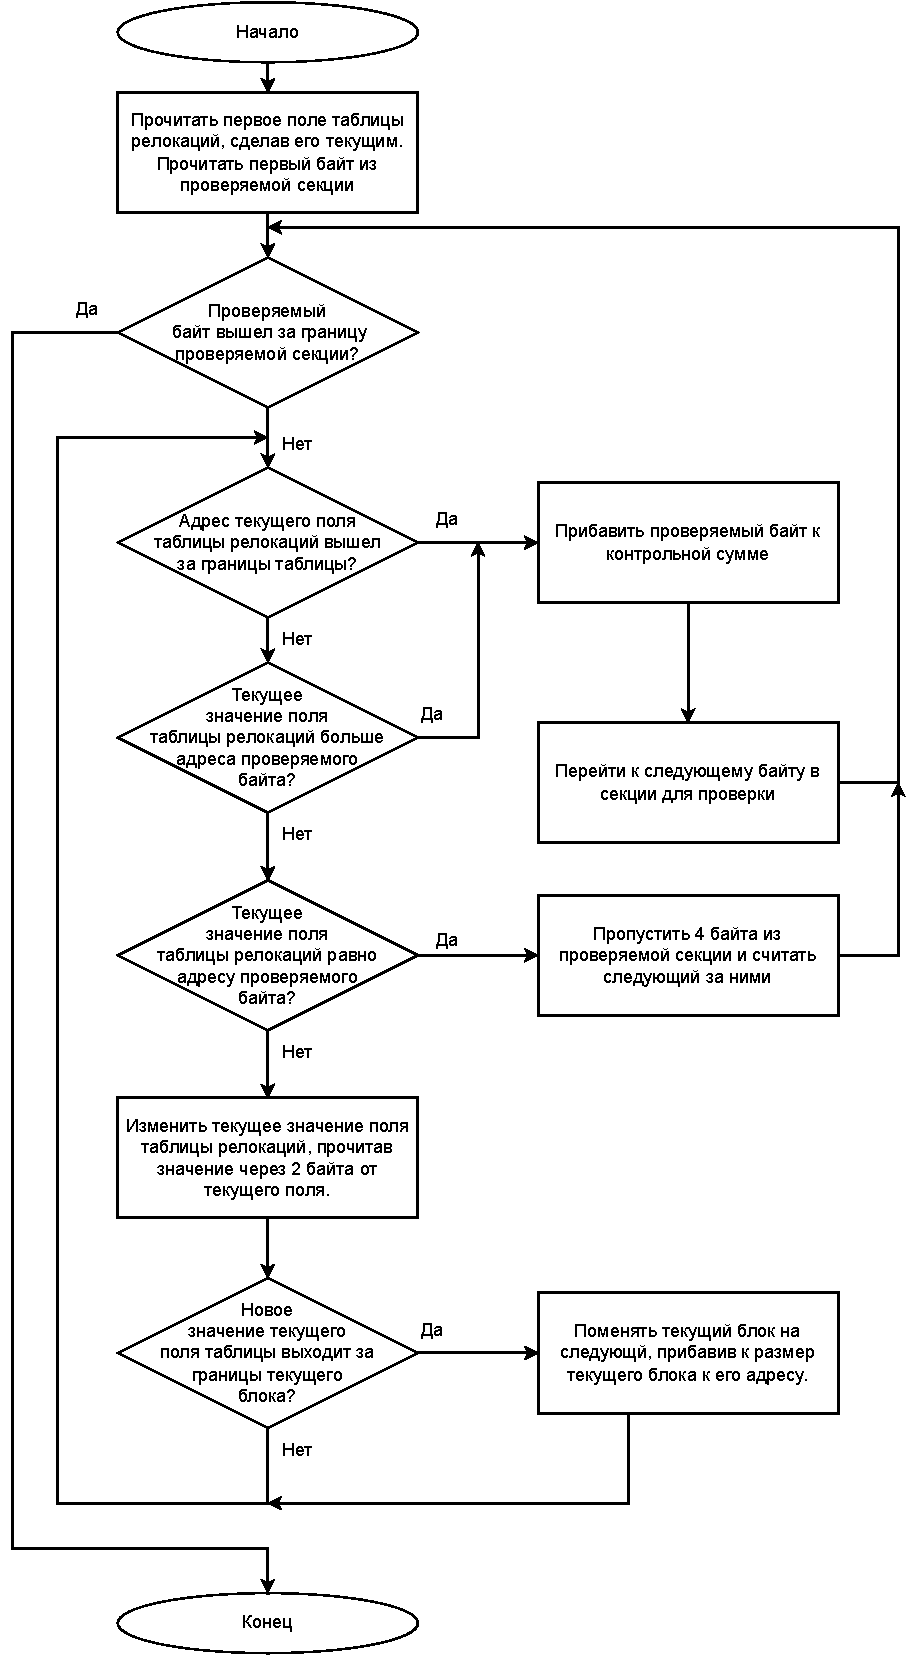
\includegraphics[height=\textheight]{algorithm.pdf}
  \caption{Блок-схема алгоритма по нахождению контрольной суммы}
  \label{fig:algorithm}
\end{figure}

\clearpage

  %! TEX root = ../../main.tex

\section{Реализация алгоритма}

В данной работе приведенный алгоритм реализован на языке ассемблера. Сам
ассемблерный код реализован в виде макроса. Преимуществом такого подхода
является то, что при вызове функции-макроса происходит не вызов функции, а
подстановка кода функции на место вызова. То есть это работает аналогично
встраиваемым функциям. Однако, если попытаться сделать функцию, содержащую код
алгоритма, встраиваемой, то компилятор проигнорирует ключевое слово
\verb!inline!. Для компилятора MSVC данная проблема решается ключевым словом
\verb!__forceinline!, но, например, если поменять компилятор на gcc, то такое
решение уже не подойдет.  Для обеспечения универсальности кода по отношению к
компилятору реализация алгоритма помещена в макрос.

Использование макроса предоставляет еще одну полезную возможность, а именно
указать при вызове разный порядок регистров. Таким образом, вызывая
макрос с разным порядком регистров, будут получаться разные участки кода. Если
злоумышленник найдет и исправит один блок защиты, то найти остальные путем
поиска повторяющихся элементов памяти у него не получится.

Объявление макроса выглядит следующим образом:
\begin{verbatim}
  #define GET_CRC(reg_A, reg_B, reg_C, \
                  reg_D, reg_SI, reg_DI, out_var) ...
\end{verbatim}
В качестве регистра при вызове макроса необходимо передать букву, которая его
обозначает. Для \verb!eax! необходимо передать \verb!a!, для \verb!ebx! ---
\verb!b! и так далее. Только для регистров \verb!esi! и \verb!edi! необходимо
передать \verb!si! и \verb!di! соответственно. Это связано с тем, что при работе
с этими регистрами невозможно обратиться к их младшему байту.

Внутри макроса имена регистров соединяются при помощи псевдооперации \verb!##!.
Так, например, строчка кода
\begin{verbatim}
  mov al, byte ptr [ebx]
\end{verbatim}
принимает вид
\begin{verbatim}
  mov reg_A##l, byte ptr [e##reg_B##x]
\end{verbatim}

При оформлении кода ассемблера в виде макроса приходится учитывать следующие
правила:
\begin{enumerate}
  \item Заключить код в \verb!__asm{...}! блок.
  \item Поместить ключевое слово \verb!__asm! перед каждой ассемблерной
    инструкцией.
  \item Использовать только блочные комментарии (\verb!/*...*/!).
\end{enumerate}
Эти правила обусловлены тем, что при подстановке макроса он всегда занимает
только одну строку.

Первое правило необходимо соблюдать, чтобы макрос можно было использовать в
одной строке с другим кодом языка C или C++. Без закрывающей фигурной скобки
компилятор не сможет понять, где заканчивается ассемблерный код, и будет
воспринимать код C или C++ как ассемблерные инструкции.

Второе правило обусловлено тем, что ключевое слово \verb!__asm! и перевод строки
являются единственными разделителями операторов в ассемблерных вставках. Из-за
того, что подстановка макроса происходит в одну строку, из доступных
разделителей операторов остается только ключевое слово \verb!__asm!.

Третье правило ограничивает использование строчных комментариев, так как первый
строчный комментарий сделает всю оставшуюся часть макроса комментарием.

Также при разработке макроса пришлось столкнуться с проблемой невозможности
установки меток внутри ассемблерной вставки. Чтобы установить метку,
необходимо закрыть блок ассемблерной вставки, установить метку и открыть новую
ассемблерную вставку.

Ниже приведен пример корректного макроса с ассемблерной вставкой.
\begin{verbatim}
  #define EXAMPLE_MACRO(out_var) __asm \
  { \
    __asm mov eax, value    /* Place value in eax */ \
    __asm cmp eax, svalue   /* compare first and second value */ \
    __asm je l1 \
    __asm mov out_var, eax \ 
    __asm jmp end \
  } \
  l1: \
  __asm { \
    __asm add eax, 0x200    /* Increase eax by 200 */ \
    __asm mov out_var, eax \
  } \
  end:
\end{verbatim}

  %! TEX root = ../main.tex

\section{Набор классов для нахождения контрольной суммы}

Помимо макроса для нахождения контрольной суммы в ходе работы были реализованы
(TODO) модули, обеспечивающие нахождение контрольной суммы различных секций 
процессов, загруженных в память и расположенных на диске.

Модули представляют из себя набор из трех классов, написанных на языке C++. Он
включает в себя:
\begin{itemize}
  \item \verb!CRC_general!--- базовый абстрактный класс, в котором реализована
    основная логика работы с секциями и алгоритм нахождения контрольной суммы.
  \item \verb!CRC_exe! --- унаследованный от \verb!CRC_general! класс,
    реализующий работу с исполняемыми файлами, расположенными на диске.
  \item \verb!CRC_image! --- унаследованный от \verb!CRC_general! класс,
    реализующий работу с исполняемыми файлами, загруженными в оперативную
    память.
\end{itemize}

Различия в работе с секциями исполняемых файлов, один из который хранится на
диске, а другой загружен в память, заключается в разных значениях смещений
внутри кода. В таблице секций PE-формата для каждой секции содержится два поля:
\verb!VirtualAddress! и \verb!PointerToRawData!. Поле \verb!VirtualAddress!
содержится относительный виртуальный адрес секции при загрузке программы в
памяти. В свою очередь, поле \verb!PointerToRawData! содержит смещение
относительно начала \textit{файла}, по которому расположена данная секция.

Еще одно отличие заключается в том, что при работе с процессом, расположенном на
диске, базовым адресом загрузки необходимо считать начало файла. При этом
необходимо учитывать, что адреса, вычисляемые по таблице релокаций,
соответствуют смещению секций не внутри файла, а внутри программы загруженной в
память.

Реализованные модули следует использовать не для организации защиты приложения,
а для скорее для отладки. В связи с этим реализованный в них алгоритм отличается
от представленного на рисунке \ref{fig:algorithm}. Для нахождения контрольной
суммы все адреса из таблицы релокаций заносятся в ассоциативный контейнер
(\verb!std::set!). При подсчеты контрольной суммы, если адрес проверяемого байта
содержится в этом контейнере, то этот и следующие за ним три байта игнорируются.
Также данные классы позволяют находить контрольную сумму любых секций. Для этого
им необходимо передать битовую маску, соответствующую характеристикам секции.

Также в данных классах реализована система логирования, настраиваемая с помощью
директив препроцессора. Так, например, можно указать файл, в который будут
записаны все значения из таблицы релокаций, или все значения байт с их адресам,
которые вошли в контрольную сумму.

Класс \verb!CRC_exe! реализует еще одну важную функцию. Защищаемая программа
после нахождения своей контрольной суммы должна сравнить ее с эталонным
значением. Эталонное значение должно хранится в другой секции данной программы.
Класс \verb!CRC_exe! позволяет записать найденное значение контрольной суммы в
файл расположенный на диске. 

Защищаемая программа должна разместить в своей памяти ключ размером в четыре
байта. Если защищаемая программа будет проверять целостность своей секции кода,
то ключ можно расположить в секции инициализированных данных (.data). Сделать
это можно путем объявления глобальной переменной, проинициализировав ее
значением ключа. Так как в коде программы значение данной переменной меняться не
будет, ее следует пометить как \verb!volatile!. Иначе компилятор может
попытаться оптимизировать обращение к данной переменной и просто подставить
значение данной переменной в код программы, вместо того чтобы читать это
значение из адреса памяти. Пример объявления такой переменной:
\begin{verbatim}
  volatile uint32_t CRC = 0x4C52454B;
\end{verbatim}

Класс \verb!CRC_exe! позволяет записать значение контрольной суммы выбранной
секции во все места, где в программе встретиться ключевое значение. Для этого
можно применить следующий код:
\begin{verbatim}
  CRC_exe crc_finder;
  uint32_t crc;
  crc_finder.read_file("file_name.exe");
  crc = crc_finder.get_sections_CRC(IMAGE_SCN_CNT_CODE);
  crc_finder.replace_all_keys(KEY, crc);
  crc_finder.write_file("new_file_name.exe");
\end{verbatim}



  \StdChapter{Тестирование программы безопасности}
  %! TEX root = ../main.tex

Для проведения тестов, была написана простая демонстрационная программа.
Программа написана на языке C с использованием WinAPI. Ее интерфейс (рисунок
\ref{fig:interface}) представляет из себя два поля \verb!edit! для логина и для
серийного ключа. Серийный ключ генерируется из имени пользователя в процессе
работы программы.

\begin{figure}[h!]
  \centering
  \begin{subfigure}[bt]{0.45\textwidth}
    \centering
    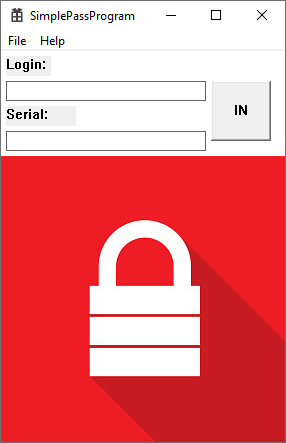
\includegraphics[width=\textwidth]{locked.png}
    \caption{}
  \end{subfigure}
  \hfill
  \begin{subfigure}[bt]{0.45\textwidth}
    \centering
    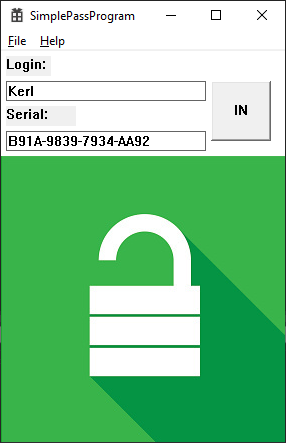
\includegraphics[width=\textwidth]{unlocked.png}
    \caption{}
  \end{subfigure}
  \caption{Интерфейс демонстрационной программы. а. --- заблокированное
    состояние; б. --- разблокированное состояние}
  \label{fig:interface}
\end{figure}

В случае, если введенный пользователем ключ не совпадает с тем, который
сгенерировала программа, выводится окно сообщения, уведомляющее пользователя о
неудаче. Данная уязвимость допущена здесь специально для большей
наглядности примера.

Для взлома данной программы воспользуемся отладчиком OllyDBG. Изменим исходный
код программы так, чтобы пользователь мог осуществить вход, введя любой пароль.

Для этого в памяти программы была найдена строка, которая выводится в окне
сообщения при неверном вводе ключа. А именно: "Invalid activation code".
Проследим по коду, предшествующему обращению к этой строке, условные переходы,
которые приводят к ситуации, когда программа остается заблокированной. Таким
образом легко обнаружить проверку двух строк на равенство. Очевидно в этом месте
происходит проверка ключа. На рисунке \ref{fig:disas_no_protect} видно, что по
адресу \verb!00FF143F! располагается проверка признака корректности ключа, после
чего идет условный переход на секцию кода, которая приводит к блокировке
приложения.

\begin{figure}[htpb]
  \centering
  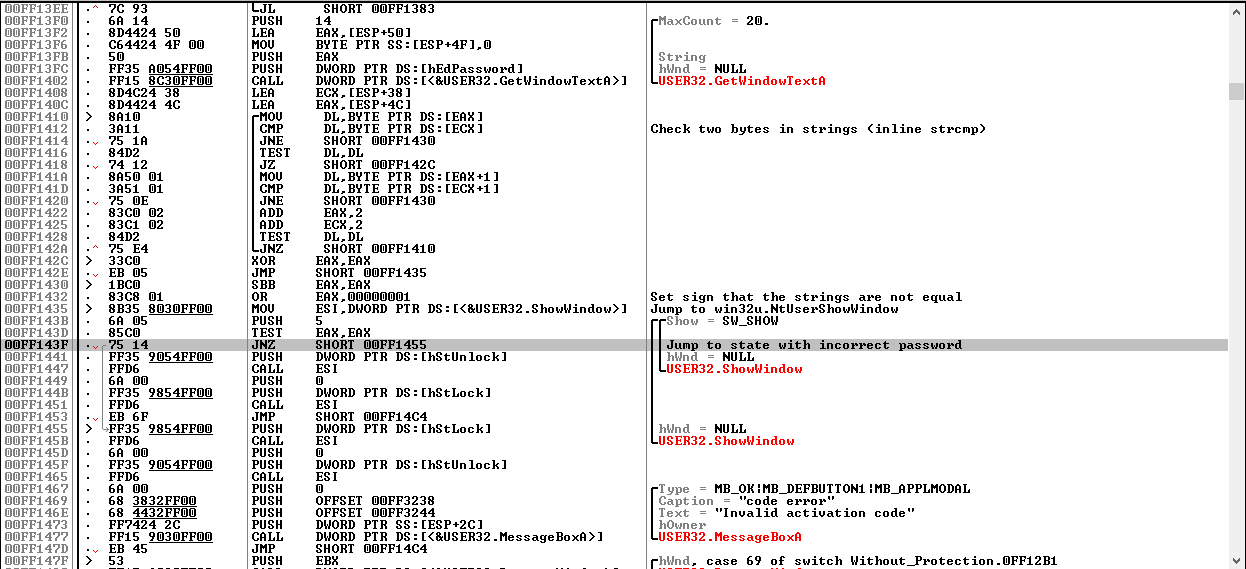
\includegraphics[width=\textwidth]{check_pass_section_croped.png}
  \caption{Окно отладчика при взломе программы без защиты}
  \label{fig:disas_no_protect}
\end{figure}

Так как наличие в регистре \verb!eax! значения отличного от нуля свидетельствует
о том, что введенный ключ не является корректным, оптимальным вариантом является
замена инструкции:
\begin{verbatim}
  test eax, eax
\end{verbatim}
на инструкцию
\begin{verbatim}
  xor eax, eax
\end{verbatim}
Таким образом в регистр \verb!eax! будет занесено значение 0, как и требует того
алгоритм программы при вводе корректного ключа. А условный переход выполняться
не будет .


На рисунке \ref{fig:cracked_unlock} представлена работа полученной таким образом
программы.
\begin{figure}[htpb]
  \centering
  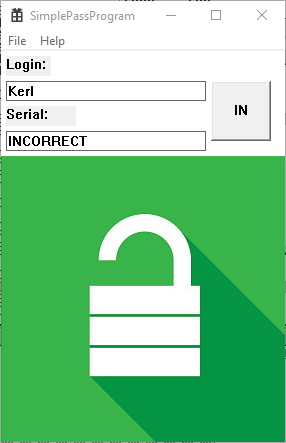
\includegraphics[width=0.4\textwidth]{cracked_unlocked.png}
  \caption{Работа взломанной программы}
  \label{fig:cracked_unlock}
\end{figure}

Теперь разместим в коде нашей программы разработанную ранее защиту от отладчика. 
Для этого создадим глобальную переменную:
\begin{verbatim}
  static const volatile DWORD CRC = 0x4C52454B;
\end{verbatim}
При помощи реализованных модулей вторая программа занесет в эту переменную
значение, равное контрольной сумме секции кода. Защиту разместим в участке кода,
который выполняется при нажатии на кнопку \verb!IN!. Если полученная контрольная
сумма не будет совпадать с эталонным значением, то будет выведено диалоговое
окно, сообщающее, что целостность кода была нарушена, а проверка пароля
выполняться не будет.

Стоит отметить, что уведомление пользователя об обнаружении отладчика или
нарушении целостности программы само по себе является уязвимостью. Такое
поведение реализовано исключительно в целях наглядности.

Исходный код программы претерпел незначительные изменения (рисунок
\ref{fig:protected_code}). Признак корректности ключа заносится в регистр
\verb!ecx! по адресу \verb!008B147B!.

\begin{figure}[htpb]
  \centering
  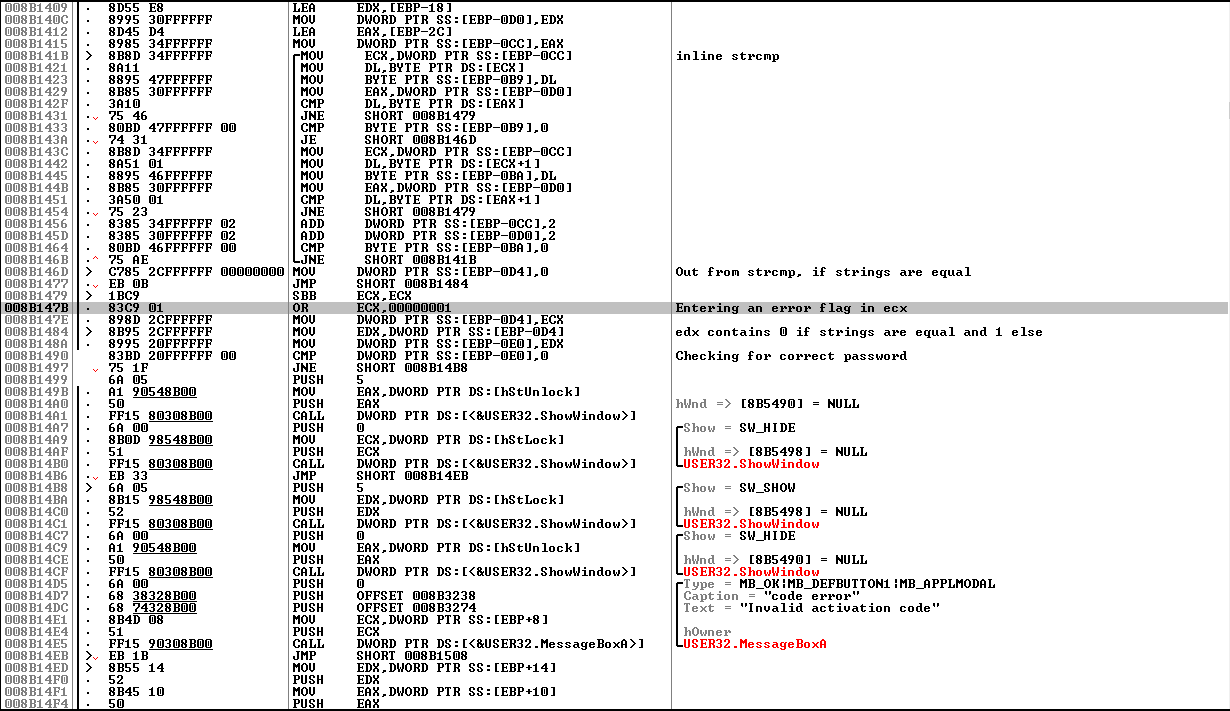
\includegraphics[width=\textwidth]{check_pass_section_protected_croped.png}
  \caption{Окно отладчика при взломе программы с защитой}
  \label{fig:protected_code}
\end{figure}

Для взлома программы заменим инструкцию
\begin{verbatim}
  or ecx, 1
\end{verbatim}
на инструкцию
\begin{verbatim}
  xor ecx, ecx  
\end{verbatim}

Так как полученная инструкция занимает на один байт меньше памяти,
освободившееся место заполним инструкцией \verb!nop!. Сохраним полученную
программу и попробуем ввести некорректное значение ключа.

\begin{figure}[hpbt]
  \centering
  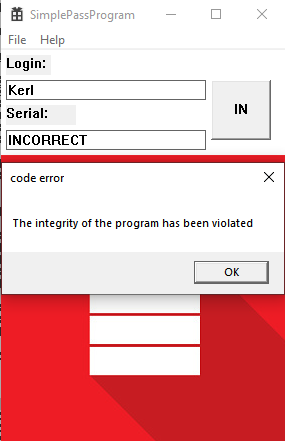
\includegraphics[width=0.4\textwidth]{Protection_work.png}
  \caption{Работа программы с защитой от взлома}
  \label{fig:protection_work}
\end{figure}

Как видно из рисунка \ref{fig:protection_work}, разработанная система
обеспечивает достойную защиту приложения.
\newpage

Также стоит отметь, что если в отладчике установить точку останова, то он
занесет в первый байт инструкции значение \verb!CC!. Таким образом контрольная
сумма кода изменится и разработанный алгоритм позволяет это обнаружить. Данная
особенность защиты проиллюстрирована на рисунке \ref{fig:break_poin_catch}.

\begin{figure}[htpb]
  \centering
  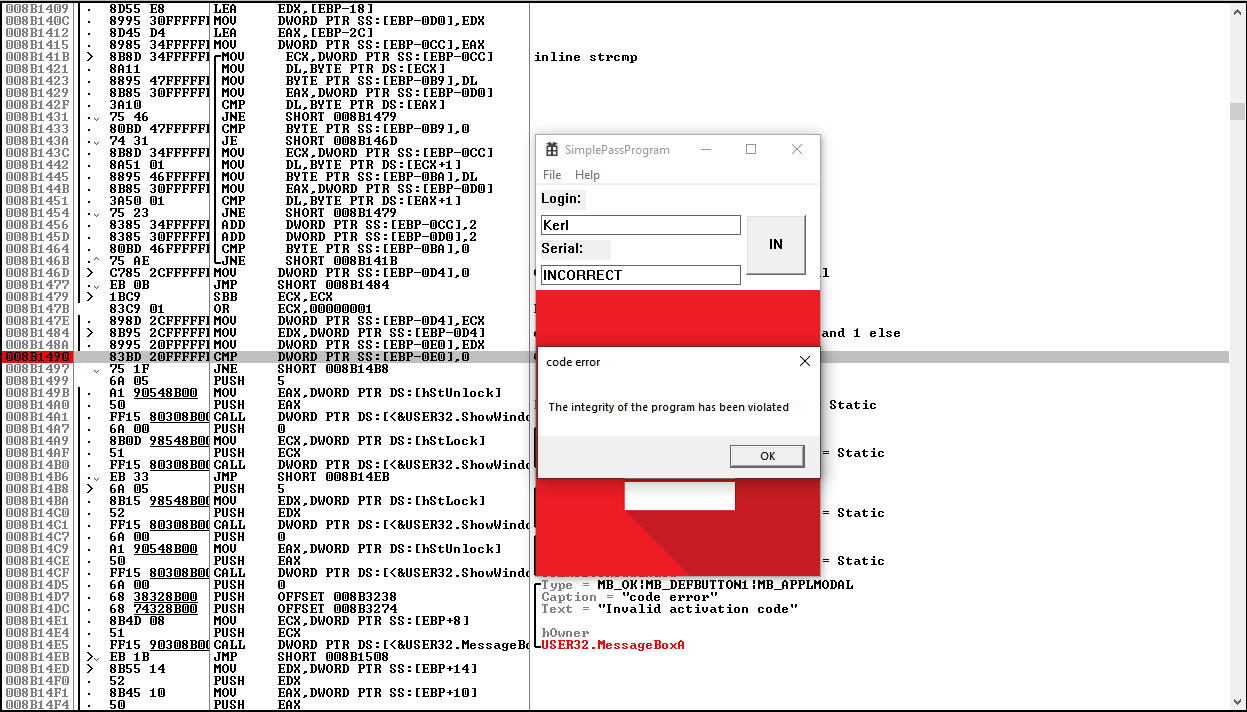
\includegraphics[width=0.8\textwidth]{Catch_breakpoint.png}
  \caption{Обнаружение системой защиты установленной точки останова}
  \label{fig:break_poin_catch}
\end{figure}

В ходе тестирования было выявлено, что при передачи различных регистров в
вызов макроса максимальная длина повторяющихся байт равна 9:
\begin{verbatim}
  0F 84 8B 00 00 00 EB EA FF
\end{verbatim}

Данные байты операции соответствуют двум инструкциям:
\begin{verbatim}
  je  no_section
  jmp section_loop
\end{verbatim}

Если повторяющаяся последовательность длинной в 9 байт покажется критичной,
можно вставить между этими инструкциями любую операцию с каким-либо регистром.
Например:
\begin{verbatim}
  xor ebx, ebx
\end{verbatim}

Результаты тестирования показывают, что реализованный метод обеспечивает защиту
программы от модификации исходного кода на должном уровне. Кроме того
реализованный метод препятствует процессу отладки. 


  \chapter*{Заключение}
  %! TEX root = ../main.tex

\section{Выводы (Слайды: 10)}

В рамках ВКР разработан метод защиты программы от изменения ее исходного кода, а
также препятствующий процессу отладки. Разработан алгоритм нахождения
контрольной суммы кода защищаемой секции. Составленный алгоритм реализован и
протестирован. Результаты тестирования показали, что разработанный метод
обеспечивает защиту на достойном уровне.

Алгоритм реализован на языке ассемблера. Ассемблерный код был помещен в макрос
языка C. Написаны программные модули на языке C++ для работы с секциями
PE-файла.



  \addcontentsline{toc}{chapter}{Заключение}

  %! TEX root = ../main.tex

\addcontentsline{toc}{chapter}{Список литературы}

\begin{thebibliography}{0}

  \bibitem{stolyarov:asm} Столяров А. В. Программирование: введение в
  профессию / А. В. Столяров. -- Москва.: МАКС Пресс, 2021. -- 707 с. -- ISBN
  978-5-317-06573-7 : Текст : непосредственный. 

  \bibitem{info-bez} Информационная безопасность: сайт. -- Москва, 2020 -- URL:
  https://searchinform.ru/informatsionnaya-bezopasnost/osnovy-ib/ (дата
  обращения: 16.04.2023). -- Режим доступа: общий. -- Текст : электронный.

  %\bibitem{winten} Windows 10 Creators Update: [Электронный ресурс]. URL:
  %https://answers.microsoft.com/ru-ru/windows/forum/windows\_10update/\%D1\%87\%D1\%82\%D0\%BE/85ef878b-7cb8-46f8-80ff-5e8530ae7d5c
  %(Дата обращения: 20.04.2023)

  %\bibitem{winapi} Windows API: [Электронный ресурс]. URL:
  %https://ru.wikipedia.org/wiki/Windows\_API (Дата обращения: 09.04.23) 

  %\bibitem{antidebugger} Anti-Debugging – A Quick Guide To Avoid Malwares And
  %Mobile App Hacks: [Электронный ресурс]. URL:
  %https://www.appsealing.com/anti-debugging/ (Дата обращения 14.03.23)

  %\bibitem{msdn} MSDN Platforms: [Электронный ресурс]. URL:
  %https://visualstudio.microsoft.com/ru/msdn-platforms/ (Дата обращения
  %15.04.2023)

  %\bibitem{mpe} Microsoft Portable Executable and Common Object File Format
  %Specification: [Электронный ресурс]: Microsoft Corporation Revision 6.0 -
  %1999. Файл pdf.

\end{thebibliography}


  \appendix
  %\pagestyle{apppages}
  %! TEX root=../main.tex

%\chapter*{Приложение А}
\StdAppendix{обязательное}
            {Таблицы с описанием структур из секции релокаций}
\label{app:tables}

\begin{table}[h!]
  \centering
  \caption{Структура блока исправлений}
  \label{tab:fixup_block}
  \begin{tabularx} {\textwidth} {
      | >{\raggedright \arraybackslash \hsize=.17\hsize}X 
      | >{\arraybackslash \hsize=.13\hsize}X
      | >{\arraybackslash \hsize=.25\hsize}X
      | >{\arraybackslash \hsize=.45\hsize}X|
    } 
    \hline 
    \textbf{Смещение} & \textbf{Размер} & \textbf{Поле} & \textbf{Значение} \\
    \hline 
    0 & 4 & Относительный виртуальный адрес страницы &
      Базовый адрес загрузки и относительный виртуальный адрес
      страницы прибавляется к каждому смещению в таблице, чтобы получить
      виртуальный адрес по которому необходимо провести исправление \\
    \hline
    4 & 4 & Размер блока исправлений &
      Общее количество байтов, занимаемых блоком исправлений, включая эту
      структуру.\\
    \hline
  \end{tabularx}  
\end{table}

\begin{table}[h!]
  \centering
  \caption{Структура поля таблицы базовых релокаций}
  \begin{tabularx}{\textwidth}{
      | >{\raggedright \arraybackslash \hsize=.17\hsize}X 
      | >{\raggedright \arraybackslash \hsize=.13\hsize}X
      | >{\arraybackslash \hsize=.25\hsize}X
      | >{\arraybackslash \hsize=.45\hsize}X|
    } 
    \hline
    \textbf{Смещение} & \textbf{Размер} & \textbf{Поле} & \textbf{Значение} \\
    \hline
    0 & 4 бита & Тип & Значение, размещенное в старших четырех битах слова, 
    указывает на тип исправления. Всего типов исправлений может быть 16. Каждый
    тип указывает, как провести коррекцию значения в памяти.\\
    \hline
    0 & 12 бит & Смещение & Значение, размещенное в младших двенадцати битах
    слова, указывает смещение относительно относительного виртуального адреса
    страницы. Это смещение указывает место, где необходимо произвести
    коррекцию. \\ 
    \hline
  \end{tabularx}
  \label{tab:fixup_field}
\end{table}


  %! TEX root = ../main.tex

\chapter{\,}

\lstinputlisting[classoffset=0, 
                 language={[Visual]C++}, deletekeywords={and, xor},
                 classoffset=1,
                 morekeywords={and,xor,mov,jmp,add,lea,cmp,je,jg,jl,jge,push,pop},
                 keywordstyle=\color{blue},
                 classoffset=0
                 ]{~/work/university/Graduate_work/code/macros.asm}



\end{document}
